\documentclass{standalone}
\usepackage{mintikz}

\begin{document}
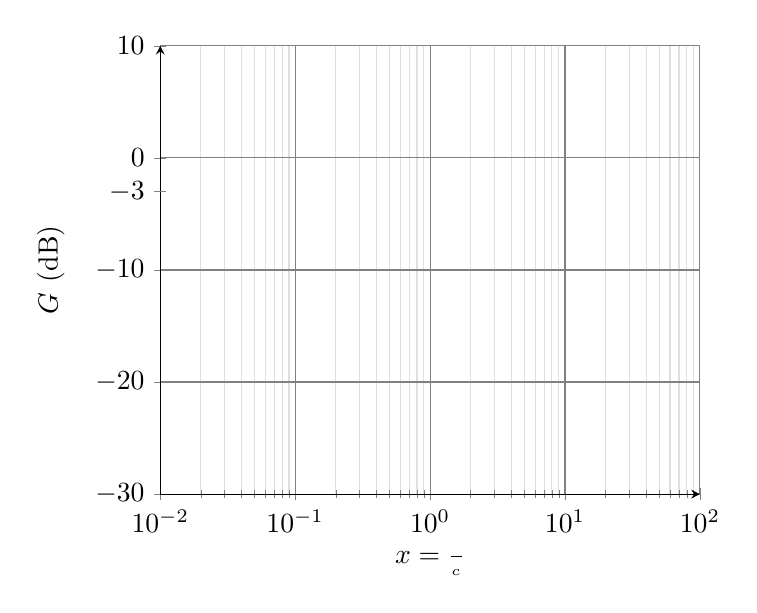
\begin{tikzpicture}[]
	\begin{semilogxaxis}[
			xmin=1e-2, xmax=1e2,
			ymin=-30, ymax=10,
			xlabel={$x=\DS\frac{\w}{\w_c}$}, ylabel=$G_{\dB}$ (dB),
			extra y ticks={-3},
			extra y tick style={grid=none},
			axis lines=left,
			grid=both,
			major grid style={black!50},
			minor grid style={gray!25},
			clip=true]
		% \addplot[
		% domain=1e-2:1e2,
		% smooth, thick, red]
		% %{log10(\x)};
		% {20*log10(1/sqrt(1+\x^2))};
		% \addplot[
		% domain=1e-2:2,
		% smooth, red, dashed, thick]
		% {0};
		% \addplot[
		% domain=6e-1:1e2,
		% smooth, red, dashed, thick]
		% {-20*log10(\x)};
		% \draw[dashed, thick]
		% (axis cs:1e-2,-3) -|
		% (axis cs:1e0,-30);
	\end{semilogxaxis}
\end{tikzpicture}
\end{document}
